\vspace{0.5cm}
\hspace{0.5cm}\textbf{1:} `ip link show` et `tc qdisc show dev h1-eth0`
\begin{center}
    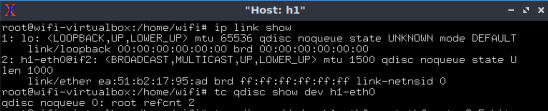
\includegraphics[width=1\textwidth]{./images/ShowDefaultQdisc.png}
\end{center}
Le résultat de ip link show indiquera si l'interface h1-eth0 est active et prête à envoyer des données, tandis que le résultat de tc qdisc show montrera les règles en place pour le contrôle du trafic, y compris les limites de bande passante et la gestion de la latence. 

\vspace{1cm}

\textbf{2:} `tc qdisc add dev h1-eth0 root handle 1:0 tbf rate 2.5gbit burst 32kbit latency 400ms (resp h2-eth0)`
\begin{center}
    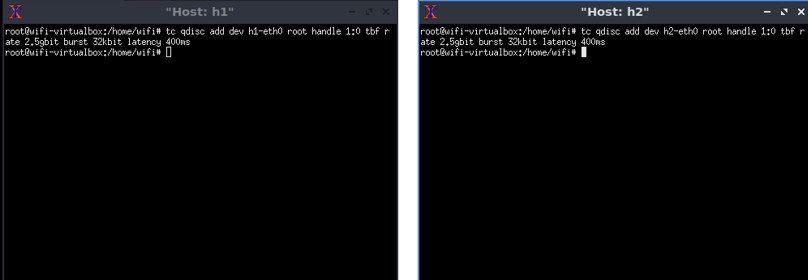
\includegraphics[width=1\textwidth]{./images/1smaller.png}
\end{center}
Les deux interfaces h1-eth0 et h2-eth0 sont configurées pour limiter le débit à 2,5 Gbps.(E1)

\vspace{1cm}
\textbf{3:} `iperf3 -s pour h1 , iperf3 -c ip-h1`
\begin{center}
    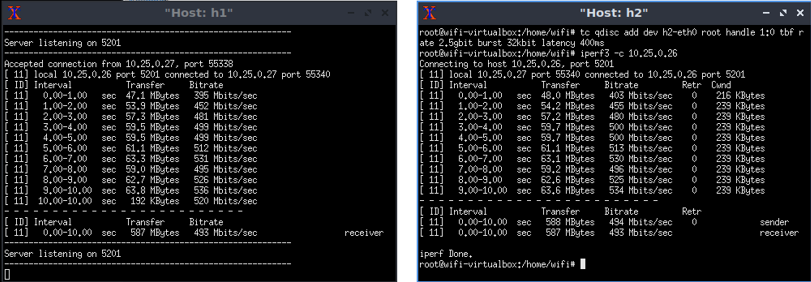
\includegraphics[width=1\textwidth]{./images/2smaller.png}
\end{center}
Pour h1 : iperf3 -s lance iperf3 en mode serveur , elle accepte la connexion au client h2\\
pour h2 : iperf3 -c 10.25.0.26 lance iperf3 en mode client et connecte au seurveur h1
\\
\\Les débits moyens de 493 Mbits/sec et 494 Mbits/sec sont observés respectivement pour le serveur et le client. Cela montre que les deux hôtes peuvent échanger des données à une vitesse proche de 500 Mbits/sec.
\\
\\Bien que les commandes tc qdisc add initiales aient fixé un débit maximum de 2,5 Gbits/sec, les résultats montrent des débits bien inférieurs à cette limite (environ 493-494 Mbits/sec).
\\ 
\\les memes tests sont fait pour une valeur moyenne (DL * 0.05) et une valeur élevée (DL par defaut), on preésente les captures : 

\vspace{1cm}
\textbf{4:} `tc qdisc add dev h1-eth0 root handle 1:0 tbf rate 125Mbit burst 32kbit latency 400ms (resp h2-eth0)`
\begin{center}
    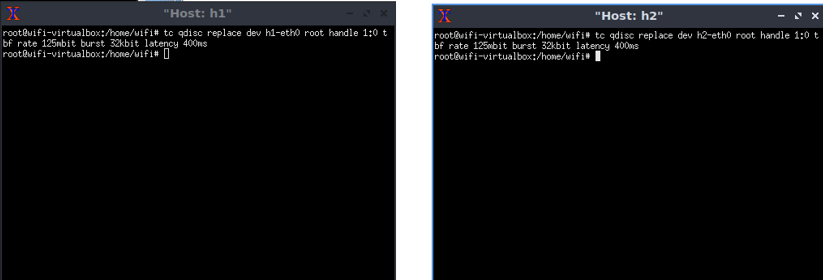
\includegraphics[width=1\textwidth]{./images/ValuerMoyenneCommande.png} \\
    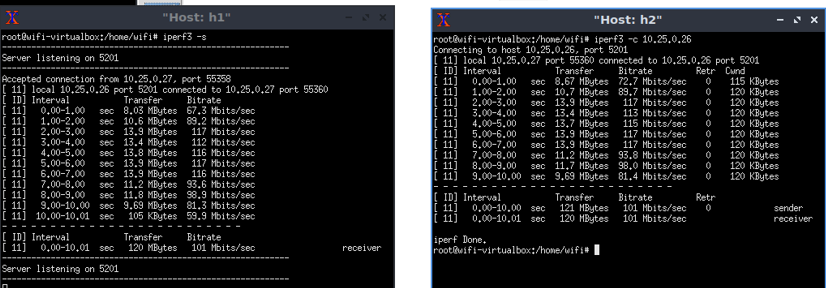
\includegraphics[width=1\textwidth]{./images/ValeurMoyenneResultat.png}
\end{center}
\vspace{1cm}
\hspace{0.5cm}\textbf{5:} `tc qdisc add dev h1-eth0 root handle 1:0 tbf rate 625Mbit burst 32kbit latency 400ms (resp h2-eth0)`
\begin{center}
    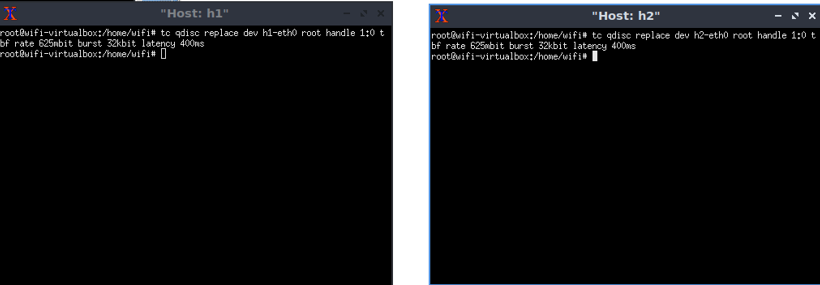
\includegraphics[width=1\textwidth]{./images/ValuerDefautCommande.png} 
    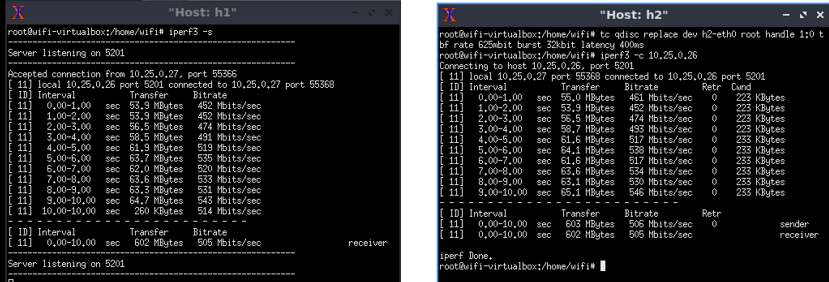
\includegraphics[width=1\textwidth]{./images/ValuerDefautResultat.png}
\end{center}
\textbf{Courbe T1.1:} 
\begin{center}
    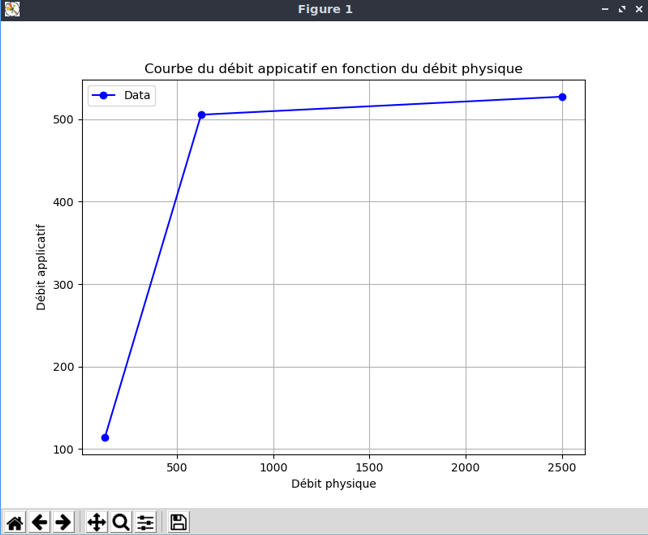
\includegraphics[width=1\textwidth]{./images/GrapheTest1.png} \\
\end{center}
Le graphe montre une relation entre le débit physique du lien (DL) et le débit applicatif mesuré lors des tests entre les machines h1 et h2.
\\
\\Le débit applicatif augmente de manière significative avec le débit physique , puis se stabilise, indiquant que d'autres facteurs, comme les limites du CPU ou l'outil iperf3 lui meme, empêchent une augmentation proportionnelle, malgré l'augmentation du débit physique.
